\begin{figure}[H]
    \caption{Basis conversion, $n < 8$}
    \begin{center}
        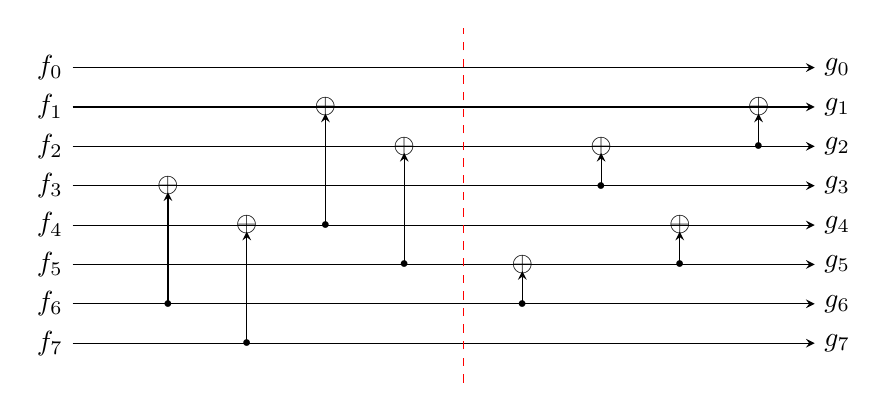
\begin{tikzpicture}[scale=0.5]
            \node (f0) at (0,7) {$f_0$};
            \node (f1) at (0,6) {$f_1$};
            \node (f2) at (0,5) {$f_2$};
            \node (f3) at (0,4) {$f_3$};
            \node (f4) at (0,3) {$f_4$};
            \node (f5) at (0,2) {$f_5$};
            \node (f6) at (0,1) {$f_6$};
            \node (f7) at (0,0) {$f_7$};
            \node (g0) at (20,7) {$g_0$};
            \node (g1) at (20,6) {$g_1$};
            \node (g2) at (20,5) {$g_2$};
            \node (g3) at (20,4) {$g_3$};
            \node (g4) at (20,3) {$g_4$};
            \node (g5) at (20,2) {$g_5$};
            \node (g6) at (20,1) {$g_6$};
            \node (g7) at (20,0) {$g_7$};

            \node (m1) at (3, 1)  {\tiny$\bullet$};
            \node (m2) at (5, 0)  {\tiny$\bullet$};
            \node (m3) at (7, 3)  {\tiny$\bullet$};
            \node (m4) at (9, 2)  {\tiny$\bullet$};
            \node (m5) at (12, 1) {\tiny$\bullet$};
            \node (m6) at (14, 4) {\tiny$\bullet$};
            \node (m7) at (16, 2) {\tiny$\bullet$};
            \node (m8) at (18, 5) {\tiny$\bullet$};

            \node (a1) at (3, 4)  {$\oplus$};
            \node (a2) at (5, 3)  {$\oplus$};
            \node (a3) at (7, 6)  {$\oplus$};
            \node (a4) at (9, 5)  {$\oplus$};
            \node (a5) at (12, 2) {$\oplus$};
            \node (a6) at (14, 5) {$\oplus$};
            \node (a7) at (16, 3) {$\oplus$};
            \node (a8) at (18, 6) {$\oplus$};

            \draw[-stealth] (f0) -- (g0);
            \draw[-stealth] (f1) -- (g1);
            \draw[-stealth] (f2) -- (g2);
            \draw[-stealth] (f3) -- (g3);
            \draw[-stealth] (f4) -- (g4);
            \draw[-stealth] (f5) -- (g5);
            \draw[-stealth] (f6) -- (g6);
            \draw[-stealth] (f7) -- (g7);

            \draw[-stealth, shorten >=-4.5pt] (m1.center) -- (a1);
            \draw[-stealth, shorten >=-4.5pt] (m2.center) -- (a2);
            \draw[-stealth, shorten >=-4.5pt] (m3.center) -- (a3);
            \draw[-stealth, shorten >=-4.5pt] (m4.center) -- (a4);
            \draw[-stealth, shorten >=-4.5pt] (m5.center) -- (a5);
            \draw[-stealth, shorten >=-4.5pt] (m6.center) -- (a6);
            \draw[-stealth, shorten >=-4.5pt] (m7.center) -- (a7);
            \draw[-stealth, shorten >=-4.5pt] (m8.center) -- (a8);

            \draw[dashed, color=red] (10.5, -1) -- (10.5, 8);

            
        \end{tikzpicture}
    \end{center}
    \label{fig:basisconv} 
\end{figure}